\documentclass[aspectratio=169,10pt]{beamer}
\usepackage[T1]{fontenc}
\usepackage{helvet}
\renewcommand{\familydefault}{\sfdefault}
\usepackage{booktabs}
\usepackage{graphicx}
\usepackage{tikz}
\usetikzlibrary{arrows.meta,positioning,fit}
\graphicspath{{../figures/}{../../demo/}}

\definecolor{ink}{HTML}{191717}
\definecolor{muted}{HTML}{5F5E5A}
\definecolor{accent}{HTML}{2A78D6}
\definecolor{warm}{HTML}{EB6834}
\definecolor{soft}{HTML}{F2F1EC}
\setbeamercolor{normal text}{fg=ink}
\setbeamercolor{frametitle}{fg=ink,bg=white}
\setbeamercolor{title}{fg=ink}
\setbeamercolor{structure}{fg=accent}
\setbeamercolor{itemize item}{fg=accent}
\setbeamercolor{enumerate item}{fg=accent}
\setbeamerfont{frametitle}{size=\Large}
\setbeamertemplate{navigation symbols}{}
\setbeamertemplate{itemize items}[circle]
\setbeamertemplate{footline}{\hfill{\color{muted}\scriptsize H\&M recommender \quad \insertframenumber/\inserttotalframenumber}\hspace{1.2em}\vspace{0.6em}}
\setlength{\leftmargini}{1.2em}

\newcommand{\stat}[2]{\begin{minipage}[t]{0.23\textwidth}{\Huge\color{accent}#1}\\[2pt]{\small\color{muted}#2}\end{minipage}}

\title{A Two-Stage Product Recommender on H\&M Data}
\subtitle{Capstone, Pillar 5: eCommerce recommendations}
\author{Matthew Martinez}
\date{October 2026 \quad\textbullet\quad github.com/mix-afk/Matthew\_Martinez\_Capstone}

\begin{document}

\begin{frame}
\titlepage
\end{frame}

\begin{frame}{Problem: pick the 12 products each customer buys next week}
\begin{columns}[T]
\begin{column}{0.52\textwidth}
\textbf{Business}
\begin{itemize}
\item 105k products, a shopper sees a few dozen
\item ``You may also like'', app home and emails default to the same best sellers
\item Goal: personalize those 12 slots, give smaller items a chance
\end{itemize}
\vspace{4pt}
\textbf{Task type}: recommendation, solved as learning to rank
\begin{enumerate}
\item Candidate generation (recall): 7 recommenders, $\sim$80 items/customer
\item Ranking: binary classifier $P(\text{buy}_{c,i,w})$, sort, take top 12
\end{enumerate}
\end{column}
\begin{column}{0.44\textwidth}
\textbf{Primary metric}: MAP@12 (Kaggle definition)
\[
\text{AP@12}(c)=\frac{1}{\min(m_c,12)}\sum_{k=1}^{12}P(k)\,\mathrm{rel}(k)
\]
\small
\textbf{Also}: Recall@12, NDCG@12, hit rate, coverage, AUC, candidate recall\\[4pt]
\textbf{Business KPIs}: CTR and add-to-cart on slots, conversion uplift vs best sellers (A/B), items per order, long-tail share of slots, hit-rate disparate impact $\geq 0.8$ per age band
\end{column}
\end{columns}
\end{frame}

\begin{frame}{Data: H\&M Personalized Fashion Recommendations (Kaggle 2022)}
\begin{columns}[T]
\begin{column}{0.5\textwidth}
\scriptsize
\begin{tabular}{lrl}
\toprule
Table & Rows & Content\\
\midrule
transactions & 31.8M & day, customer, article, price, channel\\
customers & 1.37M & age, club, newsletter flags\\
articles & 105.5k & 11 product attributes + text\\
\bottomrule
\end{tabular}
\small
\vspace{6pt}
\begin{itemize}
\item Row counts verified against the official competition
\item \textbf{Sample}: last 13 weeks, customers whose hashed id ends in \texttt{00}--\texttt{33} (20.3\%, deterministic)
\item 789k transactions, 106.7k buyers, 31.2k products
\item Missing: FN/Active 65\% (= no), age 1.2\%, club 0.4\%
\item 8.4\% exact duplicate rows = multi-unit lines (kept)
\item Price IQR outliers 3.9\% (real items, kept)
\end{itemize}
\end{column}
\begin{column}{0.48\textwidth}
\textbf{Time split} (no leakage: features use only the 8 weeks before the target week)\\[6pt]
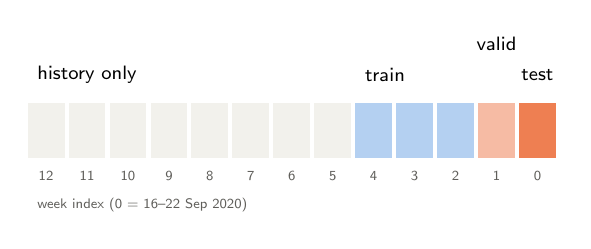
\begin{tikzpicture}[x=0.52cm,y=0.5cm]
\foreach \w/\c/\l in {12/soft/,11/soft/,10/soft/,9/soft/,8/soft/,7/soft/,6/soft/,5/soft/,4/accent!35/,3/accent!35/,2/accent!35/,1/warm!45/,0/warm!85/}{
  \fill[\c] ({12-\w},0) rectangle ({12-\w+0.9},1.4);
  \node[font=\tiny,muted] at ({12-\w+0.45},-0.45) {\w};
}
\node[font=\scriptsize,anchor=west] at (0,2.1) {history only};
\node[font=\scriptsize,anchor=west] at (8,2.1) {train};
\node[font=\scriptsize] at (11.45,2.9) {valid};
\node[font=\scriptsize] at (12.45,2.1) {test};
\node[font=\tiny,muted,anchor=west] at (0,-1.2) {week index (0 = 16--22 Sep 2020)};
\end{tikzpicture}
\vspace{6pt}
\small
\begin{itemize}
\item Train labels: weeks 2--4 (1.02M candidate rows)
\item Validation: week 1 (tuning, model choice)
\item Test: week 0, 14,023 buyers, scored once
\end{itemize}
\end{column}
\end{columns}
\end{frame}

\begin{frame}{EDA: concentrated sales, age-dependent taste, low repeat rate}
\begin{columns}[T]
\begin{column}{0.4\textwidth}
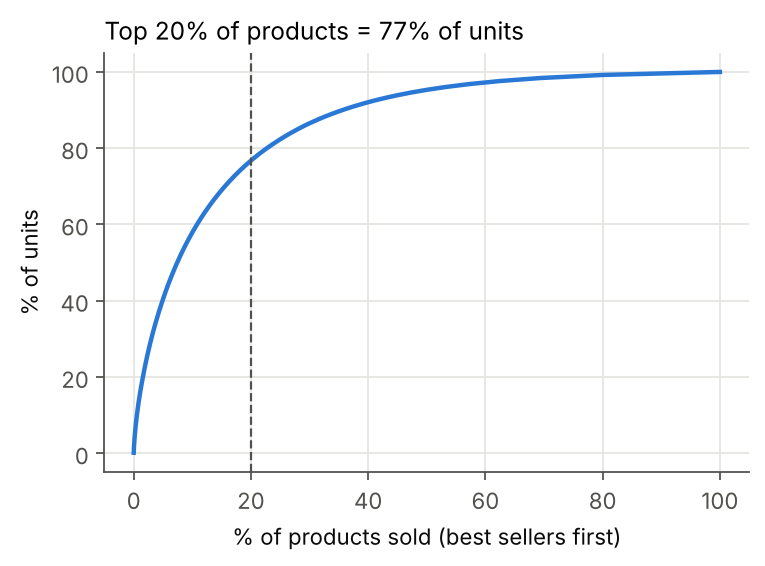
\includegraphics[width=\linewidth]{01_long_tail.png}
\end{column}
\begin{column}{0.58\textwidth}
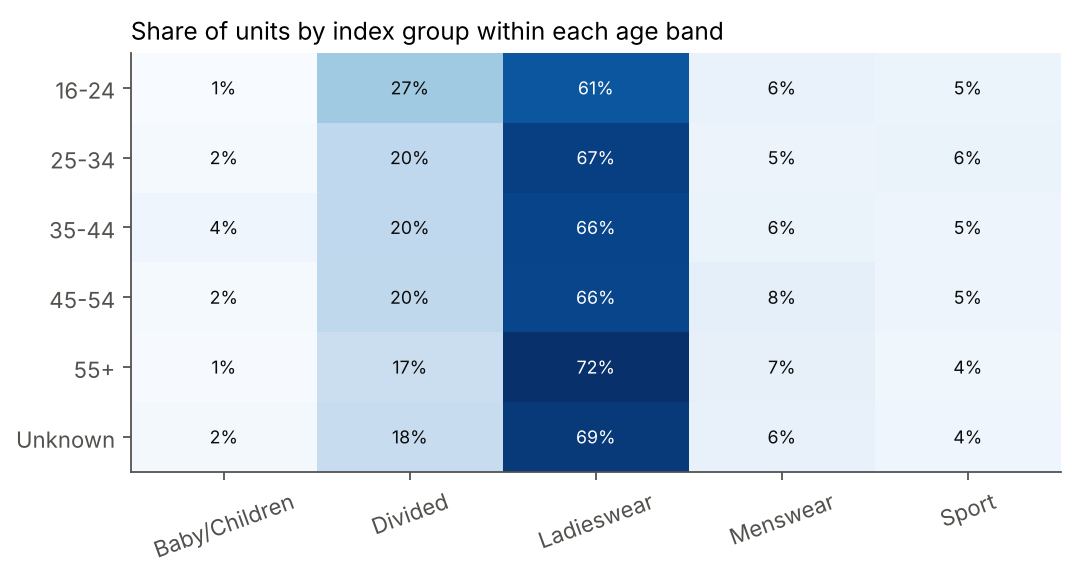
\includegraphics[width=\linewidth]{02_age_mix.png}
\end{column}
\end{columns}
\small
\begin{itemize}
\item Top 20\% of products = 77\% of units; store sales stop Mar--May 2020 (COVID), online is 70\%
\item Only \textbf{2.6\%} of next-week items were bought by the same customer in the prior 8 weeks; 4.5\% are another color of an owned product; 38\% of buyers have no 8-week history
\item Young buyers repeat less: 2.0\% repeat items for 16--24 vs 2.8\% for 55+ $\rightarrow$ expect a quality gap
\end{itemize}
\end{frame}

\begin{frame}{Pipeline}
\centering
\resizebox{\linewidth}{!}{%
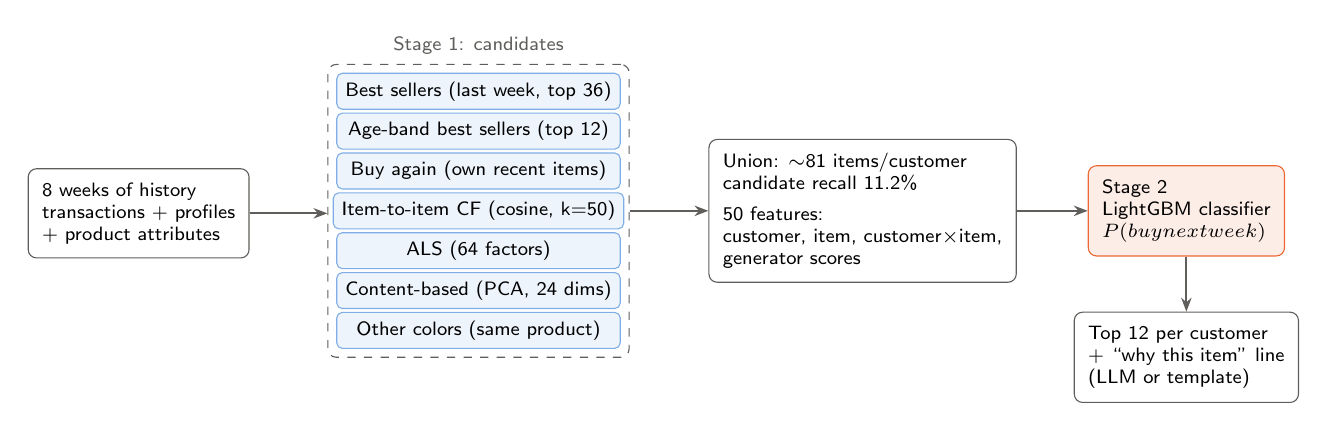
\begin{tikzpicture}[
  box/.style={draw=muted, rounded corners=3pt, fill=white, align=left, font=\scriptsize, inner sep=5pt},
  gen/.style={draw=accent!60, rounded corners=2pt, fill=accent!8, font=\scriptsize, minimum width=3.6cm, align=left, inner sep=3pt},
  arr/.style={-{Stealth[length=5pt]}, thick, color=muted}]
\node[box] (hist) {8 weeks of history\\transactions + profiles\\+ product attributes};
\node[gen, right=1.1cm of hist, yshift=1.55cm] (g1) {Best sellers (last week, top 36)};
\node[gen, below=1pt of g1] (g2) {Age-band best sellers (top 12)};
\node[gen, below=1pt of g2] (g3) {Buy again (own recent items)};
\node[gen, below=1pt of g3] (g4) {Item-to-item CF (cosine, k=50)};
\node[gen, below=1pt of g4] (g5) {ALS (64 factors)};
\node[gen, below=1pt of g5] (g6) {Content-based (PCA, 24 dims)};
\node[gen, below=1pt of g6] (g7) {Other colors (same product)};
\node[draw=muted, dashed, rounded corners=3pt, fit=(g1)(g7), inner sep=3pt, label={[font=\scriptsize,muted]above:Stage 1: candidates}] (stage1) {};
\node[box, right=1.0cm of stage1] (feat) {Union: $\sim$81 items/customer\\candidate recall 11.2\%\\[3pt] 50 features:\\customer, item, customer$\times$item,\\generator scores};
\node[box, right=0.9cm of feat, fill=warm!12, draw=warm] (rank) {Stage 2\\LightGBM classifier\\$P(\text{buy next week})$};
\node[box, below=0.7cm of rank] (out) {Top 12 per customer\\+ ``why this item'' line\\(LLM or template)};
\draw[arr] (hist) -- (stage1.west |- hist);
\draw[arr] (stage1) -- (feat);
\draw[arr] (feat) -- (rank);
\draw[arr] (rank) -- (out);
\end{tikzpicture}}
\end{frame}

\begin{frame}{Features, selection and dimensionality reduction}
\begin{columns}[T]
\begin{column}{0.5\textwidth}
\small
\textbf{50 features}, all from the 8 weeks before the target week
\begin{itemize}
\item Generator scores/ranks (11), item (11), customer (13), customer$\times$item (10), item categoricals (5)
\item Domain: other-color count, trend (1w vs 4w avg), price ratio, taste shares, age gap
\item LR: impute + missing flags + scale + one-hot; LightGBM: native categoricals
\end{itemize}
\textbf{Selection} (same LightGBM, validation week)\\[2pt]
\scriptsize
\begin{tabular}{lrr}
\toprule
Set & Feat. & MAP@12\\
\midrule
All features & 50 & 0.0301\\
Mutual information top 25 + cat. & 30 & 0.0303\\
L1 logistic (C=0.01) + cat. & 27 & 0.0291\\
\bottomrule
\end{tabular}\\[2pt]
\small Kept all 50: MI is univariate and drops 12 of 13 customer features; needed age features in-model for the fairness tests
\end{column}
\begin{column}{0.48\textwidth}
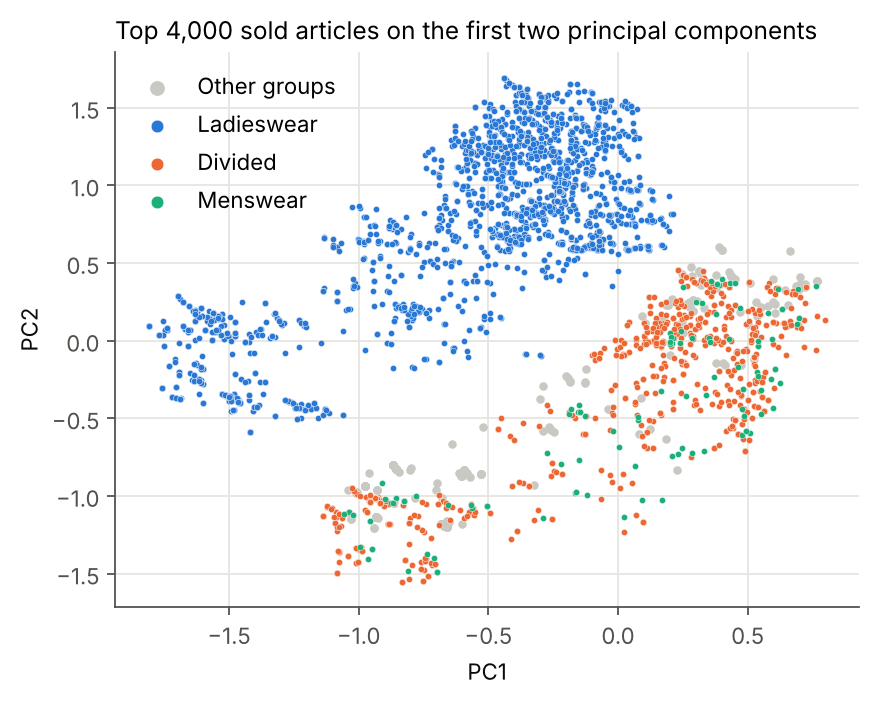
\includegraphics[width=0.49\linewidth]{02_pca_articles.png}\hfill
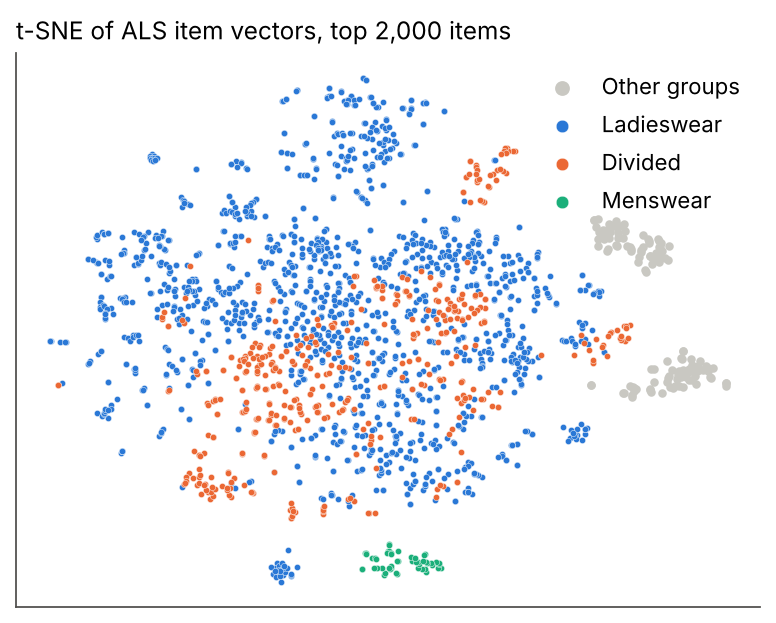
\includegraphics[width=0.49\linewidth]{02_tsne_als.png}
\small
\begin{itemize}
\item \textbf{PCA}: 600 one-hot product columns $\rightarrow$ 24 components (60\% variance), used as item vectors for content-based candidates
\item \textbf{t-SNE} of ALS item vectors: clusters by index group without seeing attributes $\rightarrow$ purchases carry style signal
\end{itemize}
\end{column}
\end{columns}
\end{frame}

\begin{frame}{Results on the held-out test week (14,023 customers)}
\begin{columns}[T]
\begin{column}{0.5\textwidth}
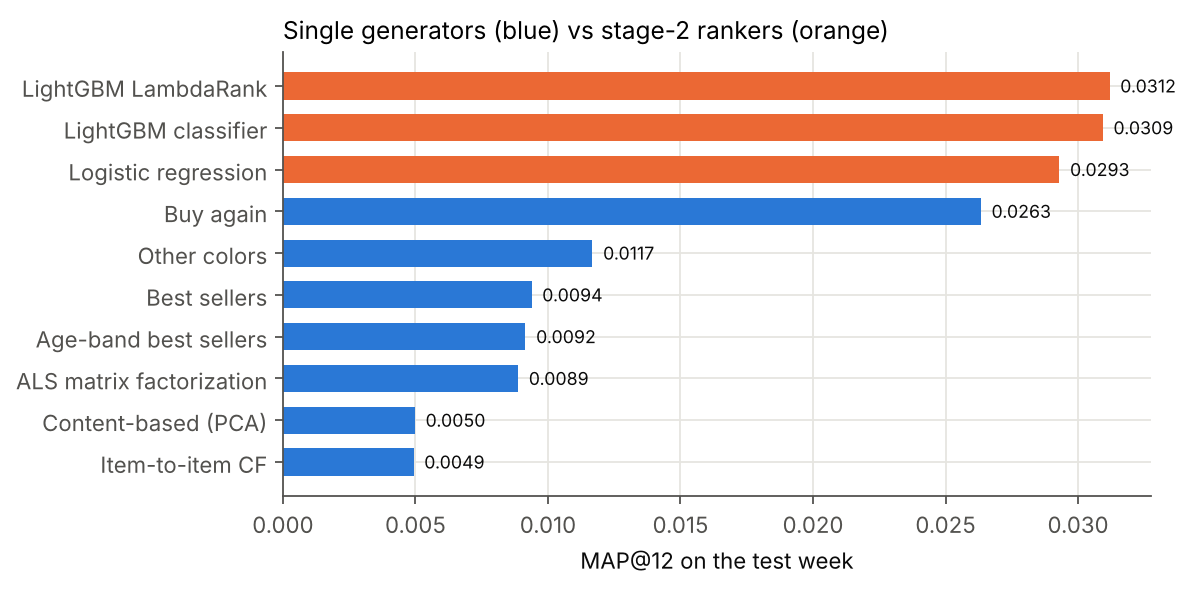
\includegraphics[width=\linewidth]{03_model_comparison.png}
\end{column}
\begin{column}{0.48\textwidth}
\scriptsize
\resizebox{\linewidth}{!}{%
\begin{tabular}{lrrrr}
\toprule
Model & MAP@12 & R@12 & Hit & AUC\\
\midrule
Best sellers & 0.0094 & 0.028 & 7.1\% & --\\
Buy again & 0.0263 & 0.056 & 11.2\% & --\\
Logistic regression & 0.0293 & 0.062 & 12.0\% & 0.730\\
\textbf{LightGBM classifier} & \textbf{0.0309} & \textbf{0.066} & \textbf{13.1\%} & \textbf{0.758}\\
LightGBM LambdaRank & 0.0312 & 0.065 & 12.7\% & 0.756\\
\bottomrule
\end{tabular}}
\small
\begin{itemize}
\item Selected on validation MAP@12 (0.0305 vs 0.0301 LambdaRank)
\item 3.3$\times$ best sellers; +17\% over the best single generator
\item LambdaRank ties MAP but loses recall, hit rate, AUC
\item Context: a top-2\% Kaggle team (45/3,006) scored 0.0300 on full data
\item Warm customers 0.0448 vs cold 0.0086 (cold $\approx$ best sellers)
\end{itemize}
\end{column}
\end{columns}
\end{frame}

\begin{frame}{Tuning and overfitting}
\begin{columns}[T]
\begin{column}{0.48\textwidth}
\small
\textbf{Tuning}: random search, 8 LightGBM settings, early stopping on validation AUC (first metric only)\\[2pt]
Best: 127 leaves, lr 0.05, min child 200, colsample 0.7, subsample 0.6, $\lambda_2$=5, 137 rounds\\[6pt]
\scriptsize
\begin{tabular}{lrrr}
\toprule
Split & MAP@12 & Hit rate & AUC\\
\midrule
Train (weeks 2--4) & 0.0420 & 16.0\% & 0.856\\
Validation (week 1) & 0.0305 & 12.7\% & 0.768\\
Test (week 0) & 0.0309 & 13.1\% & 0.758\\
\bottomrule
\end{tabular}
\small
\begin{itemize}
\item Train--valid gap: trees memorize training weeks
\item Valid $\approx$ test: generalizes to an unseen week
\item Imbalance: 0.43\% positives in test $\rightarrow$ ranking metrics, not accuracy
\end{itemize}
\end{column}
\begin{column}{0.5\textwidth}
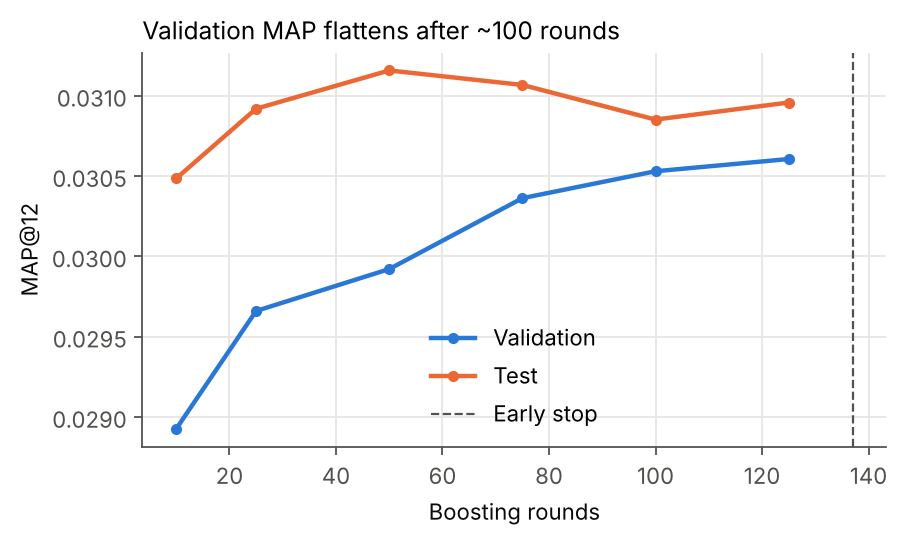
\includegraphics[width=\linewidth]{03_rounds_curve.png}
\end{column}
\end{columns}
\end{frame}

\begin{frame}{Explainability: exact TreeSHAP, PDP and ICE}
\begin{columns}[T]
\begin{column}{0.47\textwidth}
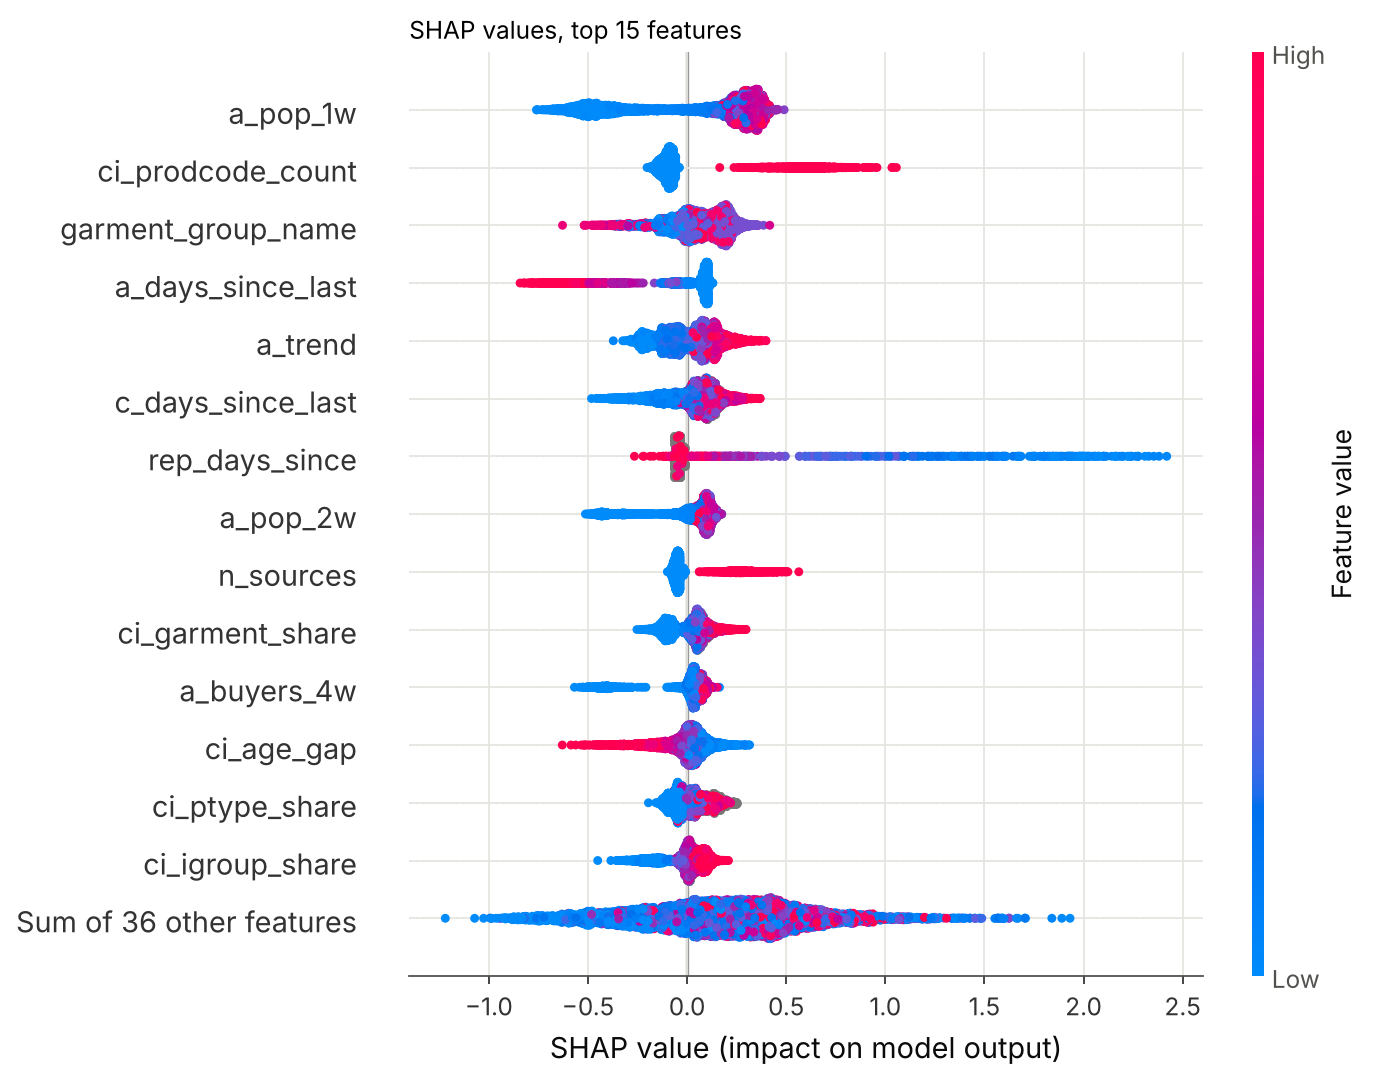
\includegraphics[width=\linewidth]{04_shap_beeswarm.png}
\end{column}
\begin{column}{0.51\textwidth}
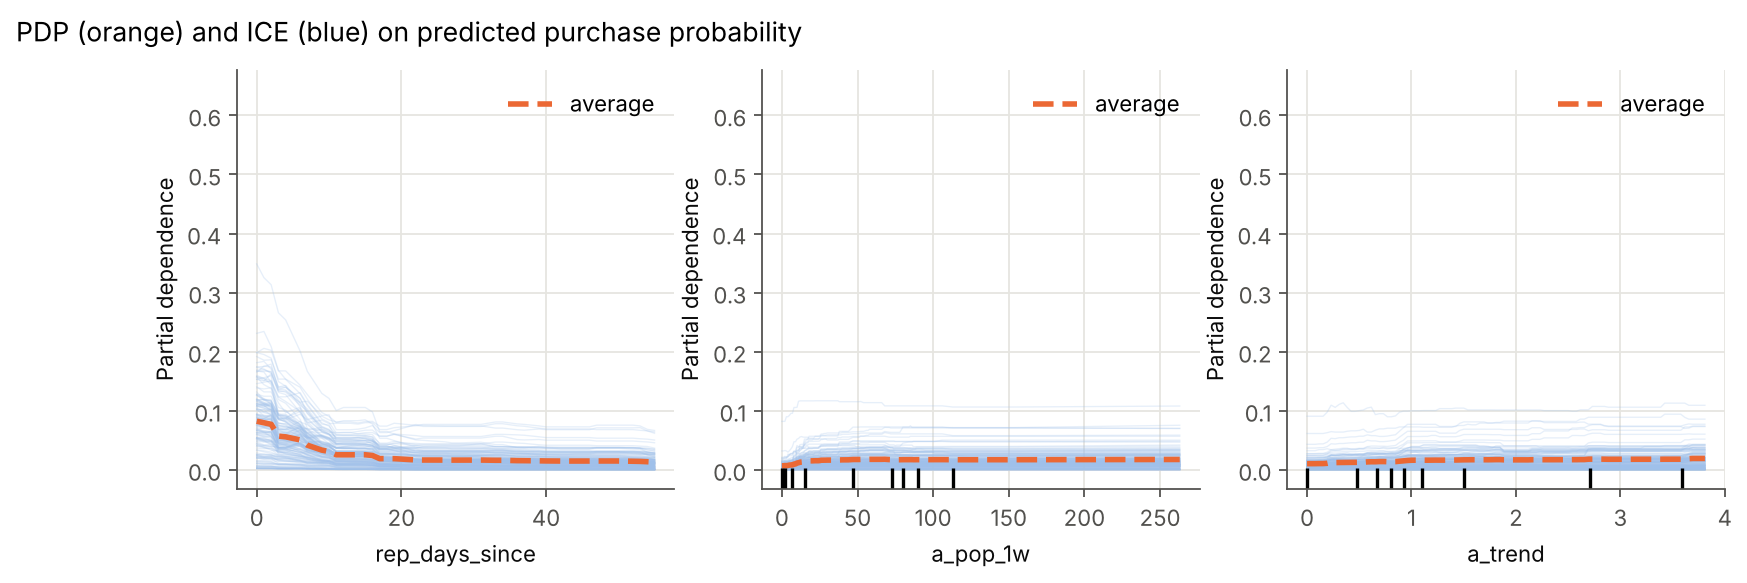
\includegraphics[width=\linewidth]{04_pdp_ice.png}
\small
\begin{itemize}
\item Top drivers: last week's sales, owning another color of the product, garment group, item and customer recency, trend
\item Bought the exact item recently: rare but the largest single effect (up to +2.4 log-odds); gain ranks it 1st, SHAP 7th
\item Age gap is 12th $\rightarrow$ how age enters the model
\item SHAP chosen over LIME: exact and stable for trees
\end{itemize}
\end{column}
\end{columns}
\end{frame}

\begin{frame}{Bias audit: age bands (customer side) and popularity (item side)}
\begin{columns}[T]
\begin{column}{0.55\textwidth}
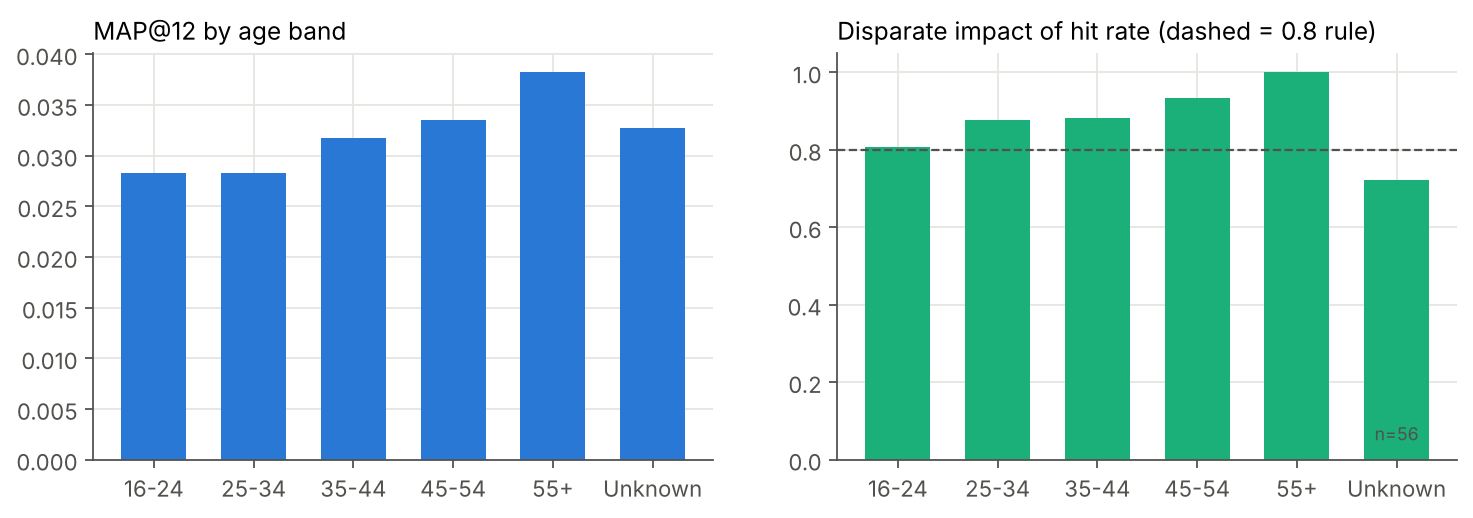
\includegraphics[width=\linewidth]{04_fairness_age.png}
\scriptsize
\begin{tabular}{lrrrr}
\toprule
Band & MAP@12 & Hit & DI & TPR\\
\midrule
16--24 & 0.0283 & 12.0\% & 0.81 & 0.450\\
25--34 & 0.0283 & 13.0\% & 0.88 & 0.434\\
35--44 & 0.0317 & 13.1\% & 0.88 & 0.429\\
45--54 & 0.0335 & 13.9\% & 0.93 & 0.475\\
55+ & 0.0382 & 14.8\% & 1.00 & 0.518\\
\bottomrule
\end{tabular}
\end{column}
\begin{column}{0.43\textwidth}
\small
\textbf{Customer side} (only age is available; gender not inferred, postal code dropped)
\begin{itemize}
\item Quality rises with age; 16--24 passes the 0.8 rule only just
\item Demographic parity diff.\ 0.012 (selection 14.1--15.3\%)
\item Equalized odds: TPR gap 0.089, FPR gap 0.012
\item Unknown band (n=56) too small to judge
\end{itemize}
\textbf{Item side}
\begin{itemize}
\item Head (top 20\% sellers) gets 95.3\% of slots; long tail is 34.1\% of purchases but 4.7\% of slots
\item Exposure Gini 0.90
\end{itemize}
\end{column}
\end{columns}
\end{frame}

\begin{frame}{Mitigations}
\begin{columns}[T]
\begin{column}{0.52\textwidth}
\scriptsize
\begin{tabular}{lrrr}
\toprule
Variant & MAP@12 & Min DI & Gap\\
\midrule
Baseline ranker & 0.0309 & 0.81 & 0.0099\\
A: reweight age bands & 0.0304 & 0.81 & 0.0118\\
B: drop age features & 0.0307 & 0.86 & 0.0096\\
C: re-rank $\lambda$=0.1 & 0.0280 & -- & --\\
\bottomrule
\end{tabular}\\[4pt]
\small
\begin{itemize}
\item A (pre-processing) did not help: young bands already the largest
\item B (unawareness): $-$0.8\% MAP, min DI 0.81 $\rightarrow$ 0.86
\item C (post-processing): long tail 4.7\% $\rightarrow$ 5.5\% of slots, coverage 29\% $\rightarrow$ 32\%, but $-$9\% MAP
\item \textbf{Ship B}; give long tail 1--2 dedicated slots instead of re-ranking; monitor DI weekly
\end{itemize}
\end{column}
\begin{column}{0.46\textwidth}
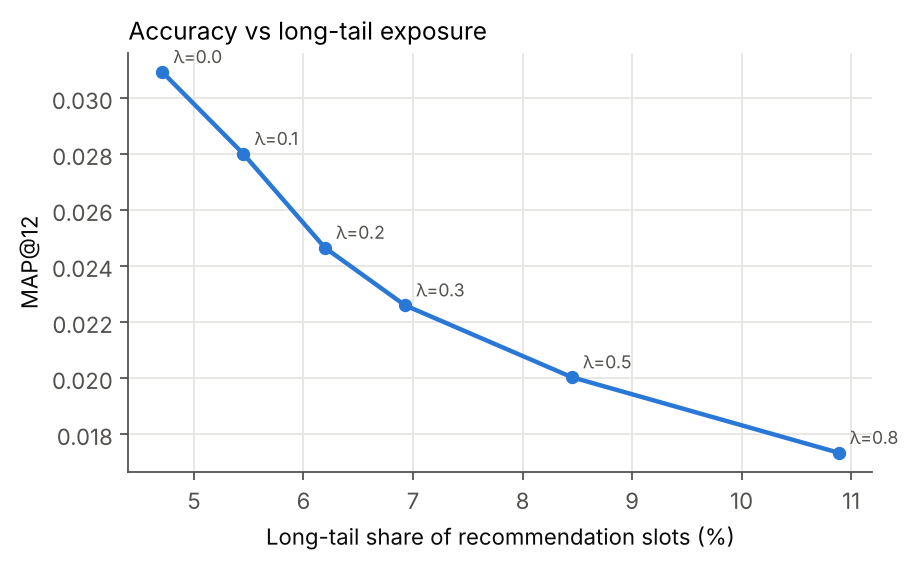
\includegraphics[width=\linewidth]{04_rerank_tradeoff.png}
\end{column}
\end{columns}
\end{frame}

\begin{frame}{Deployment, GenAI, limitations, next steps}
\begin{columns}[T]
\begin{column}{0.5\textwidth}
\small
\textbf{Serving}: nightly batch scoring $\rightarrow$ FastAPI lookup (\texttt{/recommendations}, \texttt{/similar}, \texttt{/health}), demo page, Docker, CI (ruff + 19 tests), MLflow, config-driven runs, monitoring + rollback plan\\[4pt]
\textbf{GenAI}: ranker features $\rightarrow$ facts $\rightarrow$ Claude writes a $\leq$16-word reason; guardrail blocks personal traits; template fallback without a key\\[4pt]
\textbf{Limitations}: candidate recall ceiling 11.2\%; 20\% sample; 38\% cold buyers; scaled prices, no margin; offline $\neq$ online
\end{column}
\begin{column}{0.48\textwidth}
\IfFileExists{../../demo/screenshot_recs.png}{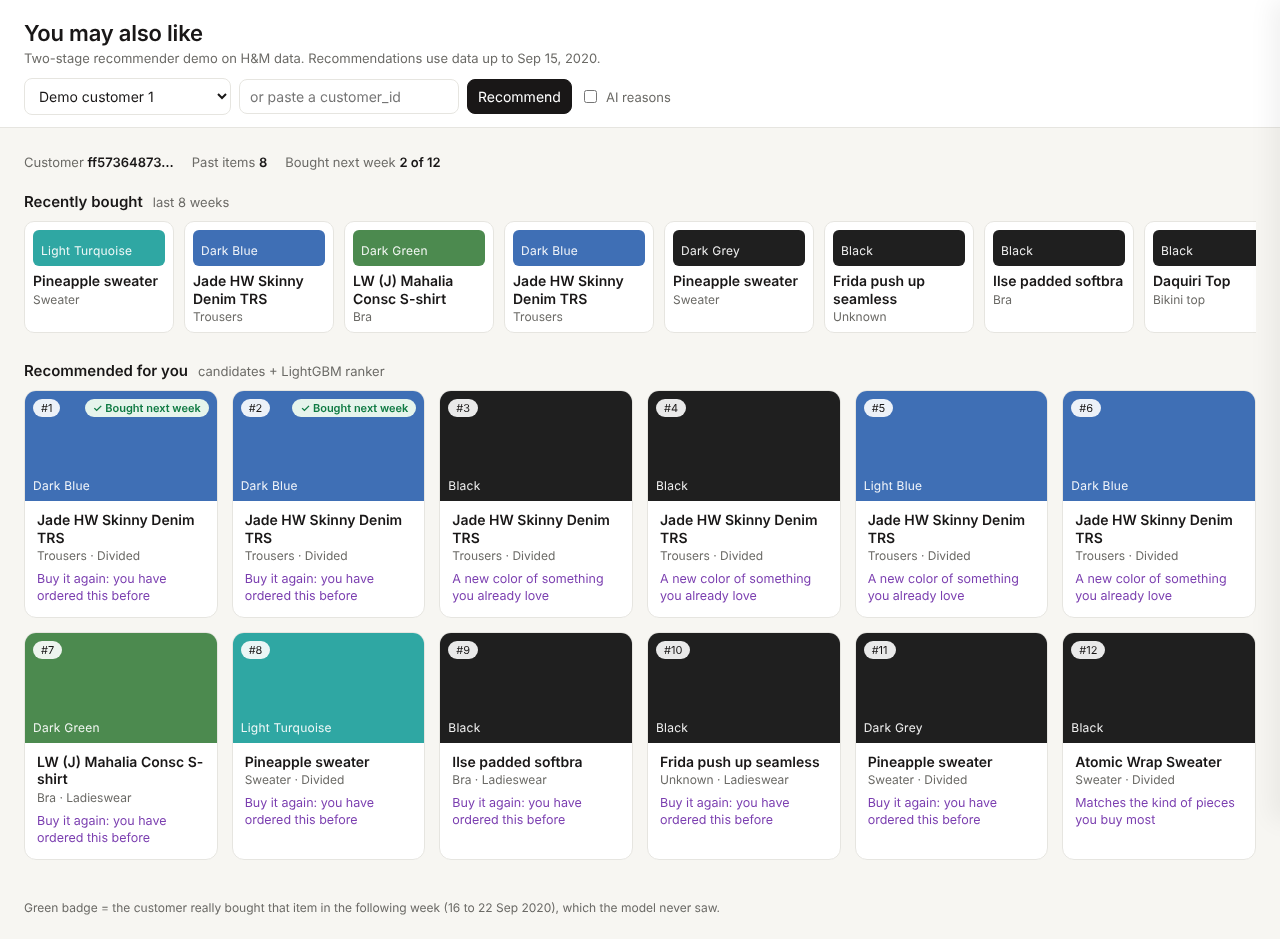
\includegraphics[width=\linewidth]{screenshot_recs.png}}{}
\small
\textbf{Next}: more candidate sources (longer window, bought-together pairs, trending in category), full data, ship variant B, A/B test vs best sellers
\end{column}
\end{columns}
\end{frame}

\end{document}
